\newpage
%%%%%%%%%%%%%%%%%%%%%%%%%%%%%%%%%%%%%%%%%%%%%%%%%%
%%%%%%%%%%%%%%%%%%%%%%%%%%%%%%%%%%%%%%%%%%%%%%%%%%
\section{Completeness proof via Sequences}
%%%%%%%%%%%%%%%%%%%%%%%%%%%%%%%%%%%%%%%%%%%%%%%%%%
%%%%%%%%%%%%%%%%%%%%%%%%%%%%%%%%%%%%%%%%%%%%%%%%%%

\begin{theorem} (completeness) $\mid$ \label{thm:completev2}
$(\Qb,\db)$ is complete.
\end{theorem}

The idea of this proof is that the real numbers are themselves sequences. The core idea is the following:

\begin{center}
\fbox{%
  \begin{minipage}{0.7\textwidth}
  \[
  \db\big([a_n],[b_n]\big) < l(\epsilon_q) \imp
  \exists N \mid \forall n \geq N,\ |a_n-b_n| < \epsilon_q
  \]
  \end{minipage}%
}
\end{center}

\begin{figure}[H]
\centering
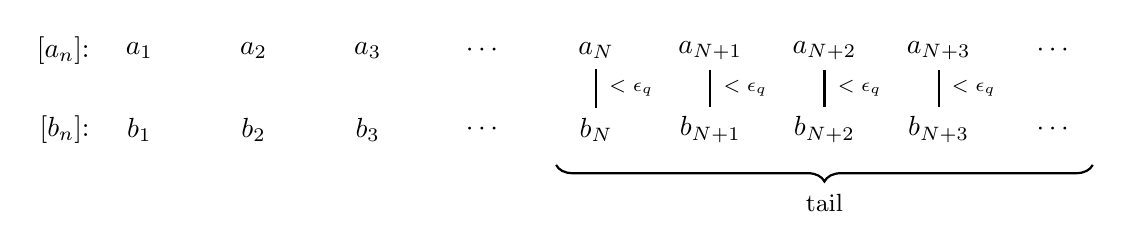
\begin{tikzpicture}[x=1.45cm,y=1cm]
  % the two sequences
  \foreach \i/\lab in {0/1,1/2,2/3} {
    \node at (\i,1) {$a_{\lab}$};
    \node at (\i,0) {$b_{\lab}$};
  }
  \node at (3,1) {$\cdots$};
  \node at (3,0) {$\cdots$};
  \foreach \i/\lab in {4/N,5/N+1,6/N+2,7/N+3} {
    \node (a\i) at (\i,1) {$a_{\lab}$};
    \node (b\i) at (\i,0) {$b_{\lab}$};
    % vertical gap |a_n - b_n| < epsilon_q
    \draw[thick] (a\i.south) -- (b\i.north)
      node[midway,right=1pt] {\scriptsize$<\epsilon_q$};
  }
  \node at (8,1) {$\cdots$};
  \node at (8,0) {$\cdots$};

  % tail: from the N-th term on
  \draw[decorate,decoration={brace,mirror,amplitude=6pt},thick]
    (3.65,-0.45) -- (8.35,-0.45)
    node[midway,below=7pt] {\small tail};

  % class brackets [a_n], [b_n]
  \node[left] at (-0.35,1) {$[a_n]\colon$};
  \node[left] at (-0.35,0) {$[b_n]\colon$};
\end{tikzpicture}
\end{figure}           

% \begin{figure}[H]
% \centering
% \begin{tikzpicture}[x=1.45cm,y=1cm]
%   % the two sequences
%   \foreach \i/\lab in {0/1,1/2,2/3} {
%     \node at (\i,1) {$a_{\lab}$};
%     \node at (\i,0) {$b_{\lab}$};
%   }
%   \node at (3,1) {$\cdots$};
%   \node at (3,0) {$\cdots$};
%   \node at (4,1) {$a_N$};
%   \node at (4,0) {$b_N$};
%   \foreach \i/\lab in {5/N+1,6/N+2,7/N+3} {
%     \node (a\i) at (\i,1) {$a_{\lab}$};
%     \node (b\i) at (\i,0) {$b_{\lab}$};
%     % vertical gap |a_n - b_n| < epsilon_q
%     \draw[thick] (a\i.south) -- (b\i.north)
%       node[midway,right=1pt] {\scriptsize$<\epsilon_q$};
%   }
%   \node at (8,1) {$\cdots$};
%   \node at (8,0) {$\cdots$};

%   % tail: from the N-th term on
%   \draw[decorate,decoration={brace,mirror,amplitude=6pt},thick]
%     (3.65,-0.45) -- (8.35,-0.45)
%     node[midway,below=7pt] {\small tail};

%   % class brackets [a_n], [b_n]
%   \node[left] at (-0.35,1) {$[a_n]\colon$};
%   \node[left] at (-0.35,0) {$[b_n]\colon$};
% \end{tikzpicture}
% \end{figure}

Let $(X_n)$ be cauchy in $(\Qb,\db)$. Use choice to get representatives
$(a_n)$ of each $X_n$ (i.e.\ each $X_n = [(a_n)]$). Explicit constructions of
these representatives are, however, possible**


%%%%%%%%%%%%%%%%%%%%%%%%%%%%%%%%%%%%%%%%%%%%%%%%%%
\subsection{Construct two sequences}

\step{1}{$(N_k): \N \to \N$.}
\begin{enumerate}[nosep,leftmargin=3em,itemsep=4pt]
    \item[(i)] $\displaystyle \forall n > N_k,\quad
        \db\Big(\big[a^{(N_k)}\big],\,\big[a^{(n)}\big]\Big) < e_k$;
    \item[(ii)] $N_k$ is the minimal such $N$.
\end{enumerate}

\paragraph{2nd idea for sequences.}
This implies that the tails are eventually all $e_k$-close.
This is exactly how we choose our $j_k$\dots

\step{2}{$(j_k): \N \to \N$.}
\begin{enumerate}[nosep,leftmargin=3em,itemsep=4pt]
    \item[(i)] $j_1 = 1$
        \hfill \textit{(doesnt rlly matter)}
    \item[(ii)] $\forall j \geq j_k,\ \ d\big(a_{j_k}^{(N_k)},\,a_{j}^{(N_k)}\big) < e_k$
        \hfill \textit{(cauchy elements)}
    \item[(iii)] $\displaystyle \forall j \ge j_{k+1},\ \
        d\Big(a^{(N_{k+1})}_{j_{k+1}},\, a^{(N_k)}_{j_{k+1}}\Big) < e_{k+1}$;
        \hfill \textit{(core idea)}
    \item[(iv)] $j_{k+1} \ge j_k$;
        \hfill \textit{(monotomically increasing)}
    \item[(v)] $j_{k+1}$ is minimal subject to (ii) \& (iii) \& (iv)
        \hfill \textit{(no choice).}
\end{enumerate}

\medskip
As I now show, it intuitively follows from a picture of our cauchy sequence as a sequence of
sequences that $\big[(a_{j_k}^{(N_k)})_{k=1}^{\infty}\big]$ gives us an element of $\Qb$ that the sequence $(X_n)$ converges to in the $(\Qb,\bar{d})$ metric.  

\begin{lemma} (geometric series) $\mid$ \label{lem:geom}
For all $B\ge0$ and $m\ge1$,
$e_B+e_{B+1}+\cdots+e_{B+m-1}\;\le\;2e_B-e_{B+m-1}\;<\;2e_B$.
\end{lemma}


%\vspace{2em}

%%%%%%%%%%%%%%%%%%%%%%%%%%%%%%%%%%%%%%%%%%%%%%%%%%
\newpage % <- Step 1 and Step 2 together on one page
\step{1}{$[(a_{j_k}^{(N_k)})_{k \in \N}]$ is cauchy \dots} 

We prove this by method of drawing a hangman


\begin{center}
% scaled to a fixed height (as big as fits with everything on one page)
\resizebox{!}{0.33\textheight}{%
\begin{tikzpicture}[x=1.9cm,y=1.1cm,>={Stealth[length=5pt]},
    dots/.style={loosely dotted,thick,shorten <=5pt,shorten >=5pt}]
  % row N_k:  a_1  a_2 ...... a_{j_k} ...... a_{j_{k+n}}
  \node (r0c1) at (0,0) {$a_1^{(N_k)}$};
  \node (r0c2) at (1,0) {$a_2^{(N_k)}$};
  \node (r0jk) at (3,0) {$a_{j_k}^{(N_k)}$};
  \node (r0jn) at (5,0) {$a_{j_{k+n}}^{(N_k)}$};
  \draw[dots] (r0c2) -- (r0jk);
  \draw[dots] (r0jk) -- (r0jn);

  % rows N_{k+1}, N_{k+2}, N_{k+3}:  a_1  a_2 ............ a_{j_{k+n}}
  \foreach \r/\lab in {1/k+1,2/k+2,3/k+3} {
    \node (r\r c1) at (0,-\r) {$a_1^{(N_{\lab})}$};
    \node (r\r c2) at (1,-\r) {$a_2^{(N_{\lab})}$};
    \node (r\r jn) at (5,-\r) {$a_{j_{k+n}}^{(N_{\lab})}$};
    \draw[dots] (r\r c2) -- (r\r jn);
  }

  % row N_{k+n}
  \node (r5c1) at (0,-5) {$a_1^{(N_{k+n})}$};
  \node (r5c2) at (1,-5) {$a_2^{(N_{k+n})}$};
  \node (r5jn) at (5,-5) {$a_{j_{k+n}}^{(N_{k+n})}$};
  \draw[dots] (r5c2) -- (r5jn);

  % vertical dots between row N_{k+3} and row N_{k+n}
  \draw[dots] (r3c1) -- (r5c1);
  \draw[dots] (r3c2) -- (r5c2);
  \draw[dots] (r3jn) -- (r5jn);
  \node at (6.15,-4) {$\vdots$};

  % top arrow:  a_{j_{k+n}}^{(N_k)} -> a_{j_k}^{(N_k)}
  \draw[->,thick] (r0jn.north) to[bend right=30]
    node[midway,above] {$<\epsilon_k$} (r0jk.north);

  % arrows up the last column, each into the row above
  \foreach \lo/\hi/\lab in {1/0/k+1,2/1/k+2,3/2/k+3} {
    \draw[->,thick] (r\lo jn.east) to[bend right=60]
      node[midway,right=2pt] {$<\epsilon_{\lab}$} (r\hi jn.east);
  }
  \draw[->,thick] (r5jn.east) to[bend right=60]
    node[midway,right=2pt] {$<\epsilon_{k+n}$} ($(r5jn.east)+(0,0.8)$);
\end{tikzpicture}%
}
\end{center}

\begin{align*}
d\big(a_{j_k}^{(N_k)},\,a_{j_{k+n}}^{(N_{k+n})}\big)
  &< \sum_{m=0}^{n} e_{k+m}
\intertext{which, by our geometric series lemma, will be, for ALL $n$, \dots}
  &< 2e_k
\end{align*}


%%%%%%%%%%%%%%%%%%%%%%%%%%%%%%%%%%%%%%%%%%%%%%%%%%

\begingroup
\setlength{\fboxsep}{12pt}                               % <- padding of the big box

\noindent
\fbox{%                                                  % <- box opens
  \begin{minipage}{\dimexpr\textwidth-2\fboxsep-2\fboxrule\relax}
  
\step{2}{prove convergence}

It suffices to show that $[(a^{(N_k)}]$ is $l(2e_k)$ close to
$\big[(a^{(N_k)}_{j_k})_{k \in \N}\big]$. Because $[(a^{(N_k)}]$ is cauchy, it
will suffice to show that a subsequence of it is eventually $(e_k)$ close.
Simply consider $(a^{N_k}_{j_{k+n}})_{n \in \N}$ and the result immediately
follows from our core idea\dots

\begin{center}
% scaled to a fixed height (as big as fits with everything on one page)
\resizebox{!}{0.24\textheight}{%
\begin{tikzpicture}[x=1.6cm,y=1.4cm,>={Stealth[length=5pt]},
    dots/.style={loosely dotted,thick,shorten <=5pt,shorten >=5pt}]
  % row N_k:  a_1  a_2 ... a_{j_k} ... a_{j_{k+1}} ... a_{j_{k+2}} ... a_{j_{k+3}} ...
  \node (c1) at (0,0) {$a_1^{(N_k)}$};
  \node (c2) at (1,0) {$a_2^{(N_k)}$};
  \node (jk) at (2.5,0) {$a_{j_k}^{(N_k)}$};
  \node (j1) at (4,0) {$a_{j_{k+1}}^{(N_k)}$};
  \node (j2) at (5.5,0) {$a_{j_{k+2}}^{(N_k)}$};
  \node (j3) at (7,0) {$a_{j_{k+3}}^{(N_k)}$};
  \coordinate (end) at (8,0);
  \draw[dots] (c2) -- (jk);
  \draw[dots] (jk) -- (j1);
  \draw[dots] (j1) -- (j2);
  \draw[dots] (j2) -- (j3);
  \draw[dots,shorten >=0pt] (j3) -- (end);

  \node[below=2pt] at (jk.south) {$(0<e_k)$};

  % staircase: a_{j_{k+i}}^{(N_k)} <-> a_{j_{k+i}}^{(N_{k+i})}
  \node (b1) at (4,-1)   {$a_{j_{k+1}}^{(N_{k+1})}$};
  \node (b2) at (5.5,-2) {$a_{j_{k+2}}^{(N_{k+2})}$};
  \node (b3) at (7,-3)   {$a_{j_{k+3}}^{(N_{k+3})}$};
  \foreach \t/\b in {j1/b1,j2/b2,j3/b3} {
    \draw[<->,thick] (\t.south) -- (\b.north)
      node[midway,right=2pt] {$<e_k$};
  }
\end{tikzpicture}%
}
\end{center}
Note that we actually don't even need step one because a sequence equivalent to a cauchy one is automatically cauchy. All we need is the proof the $<e_k$ terms which is already apparent from the same diagram of a sequence of sequences. The entire proof is contained in this diagram.

\end{minipage}%
}

\endgroup



